\documentclass[journal]{IEEEtran}
\usepackage[utf8]{inputenc} % Codificación de entrada UTF-8
\usepackage{cite} % Para citaciones
\usepackage{placeins} % Para \FloatBarrier
\usepackage{graphicx} % Para incluir imágenes
\usepackage{float}
\usepackage{amsmath} % Para fórmulas matemáticas
\usepackage{url} % Para manejar URLs
\usepackage{listings}
\usepackage{xcolor}
\usepackage[ruled,vlined]{algorithm2e} % Para pseudocódigo
\usepackage{authblk}
\usepackage{hyperref}
\usepackage{breakurl}
\usepackage[spanish]{babel}

% Configuración de listings para bash
\lstdefinelanguage{VMDPP}{
  morekeywords={class, instance, variables, private, operations, public, end, inv, is, subclass, of, bool, nat, nat1, char, real, seq, protected},
  sensitive=true,
  morecomment=[l]{//},
  morestring=[b]"
}

\lstset{
  language=VMDPP,
  basicstyle=\ttfamily\scriptsize,
  keywordstyle=\color{black}\bfseries,
  commentstyle=\color{gray},
  stringstyle=\color{blue!60!black},
  backgroundcolor=\color{white},
  numbers=left,
  numberstyle=\tiny\color{gray},
  stepnumber=1,
  numbersep=6pt,                  % <--- ajusta este valor
  xleftmargin=2em,                % <--- ¡esto mueve todo el bloque hacia la derecha!
  frame=single,
  rulecolor=\color{black!30},
  breaklines=true,
  breakatwhitespace=true,
  showstringspaces=false,
  captionpos=b
}


\title{Especificación Formal y Validación para la Prevención de Colisiones en Tráfico Ferroviario}
\author[1]{Infanzón Acosta R. E.}
\author[1]{Aguilar Chirinos C. D.}
\affil{Universidad La Salle, Arequipa, Perú}



\author[2]{Molina Barriga M. - Mentor }

\begin{document} 

\maketitle

\begin{abstract}
Aquí el Abtract o resumen
\end{abstract}

\begin{IEEEkeywords}
Aquí las Keywords
\end{IEEEkeywords}

\section{Introducción}  
La seguridad en el transporte ferroviario es un aspecto crítico para garantizar el bienestar de las personas que utilizan este medio de transporte a diario. Según el \textit{Informe sobre la Seguridad y la Interoperabilidad Ferroviaria en la UE 2024}, el sistema ferroviario de la UE se considera uno de los más seguros del mundo. Sin embargo, a pesar de la disminución de accidentes significativos desde 2010, se ha registrado un aumento en 2021 y 2022, alineándose con los niveles pre-pandemia de COVID-19. Esta realidad se ve agravada por el estancamiento de las tasas de fatalidades de pasajeros desde 2017 \cite{eu2024}. Las repercusiones de estos incidentes se extienden más allá de los pasajeros y trabajadores, afectando profundamente a las comunidades y economías que dependen del ferrocarril \cite{carrington2019}.  

Ante esta situación, es fundamental explorar nuevas estrategias para prevenir colisiones y reforzar un sistema más seguro. La implementación de tecnologías avanzadas en el ámbito de la seguridad ferroviaria se ha convertido en una prioridad. Investigaciones recientes indican que la evolución de las tecnologías de seguridad está proporcionando respuestas más efectivas ante situaciones peligrosas \cite{decel2021safety}. En este contexto, se busca desarrollar un mecanismo que minimice el riesgo de colisiones y reduzca los errores humanos y las fallas en la comunicación dentro del sistema ferroviario. La automatización de tareas críticas, como la detección de trenes en las vías y el control de su velocidad, es esencial para una respuesta adecuada ante situaciones potencialmente peligrosas \cite{automation2020}.  

Además, será necesario diseñar un modelo formal que estructure y analice la información relacionada con la seguridad ferroviaria, asegurando así la precisión y la integridad de los datos utilizados en la prevención de colisiones. Este enfoque permitirá mejorar la identificación de situaciones de riesgo y sentar las bases para futuras herramientas de mejora en la seguridad ferroviaria.  

\subsection{Alcance esperado}
El alcance de este proyecto se centra en la aplicación de métodos formales para estructurar y analizar el sistema de prevención de colisiones ferroviarias. A través del uso de VDM++ y model-checking, se busca desarrollar un modelo formal que permita verificar la consistencia y validez de las interacciones entre los componentes del sistema, como los trenes y sensores. Este enfoque garantizará la integridad de las decisiones automatizadas, como los cambios de señales o ajustes de velocidad, y asegurará que el sistema funcione correctamente en todas las condiciones posibles. Mediante un análisis riguroso y sistemático, se contribuirá a mejorar la seguridad del tráfico ferroviario, proporcionando una base sólida para el desarrollo de herramientas futuras que optimicen la prevención de accidentes en el ámbito ferroviario.

\section{Resumen Ejecutivo}

\subsection{Antecedentes}
\subsubsection{Un Sistema de Seguridad y Prevención de Colisiones en Tiempo Real para Trenes}
\subsubsection*{Resumen}  
El artículo presenta un sistema integral de seguridad que combina diversas tecnologías avanzadas para la prevención de colisiones en el transporte ferroviario. Reconoce que, a pesar de las mejoras en la infraestructura y las técnicas de gestión, los peligros persisten, lo que justifica la implementación de un enfoque más proactivo. El sistema propuesto utiliza datos en tiempo real para detectar y responder a situaciones de riesgo, con el fin de prevenir accidentes antes de que ocurran. Además, se subraya la importancia de la comunicación entre trenes, estaciones y otros elementos del sistema para asegurar una operación sincronizada y segura.
\subsubsection*{Puntos de interés para la investigación}  
\begin{itemize}
    \item \textbf{Detección y Respuesta en Tiempo Real:}  
    Según Wu (2017), el sistema se basa en tecnologías de detección que permiten identificar situaciones peligrosas en tiempo real, activando respuestas automáticas como la reducción de velocidad o la detención total antes de que se produzca una colisión \cite{railwaycouncil2017realsafetysystem}.    
    \item \textbf{Integración de Tecnologías Avanzadas:}  
    Wu (2017) destaca que se integran tecnologías como el monitoreo por GPS, sensores de proximidad y sistemas de comunicación entre trenes, lo que mejora la conciencia situacional y la capacidad de respuesta ante emergencias \cite{railwaycouncil2017realsafetysystem}.    
    \item \textbf{Comunicaciones Eficientes:}  
    Según Wu (2017), la comunicación efectiva entre los trenes y las estaciones es clave para coordinar acciones y minimizar riesgos. El autor resalta la necesidad de protocolos de comunicación robustos para asegurar que la información crítica se transmita sin demora \cite{railwaycouncil2017realsafetysystem}.   
    \item \textbf{Beneficios Socioeconómicos:}  
    Wu (2017) señala que, al reducir la frecuencia y severidad de los accidentes, el sistema no solo mejora la seguridad de los pasajeros y el personal, sino que también tiene beneficios económicos para las comunidades dependientes del transporte ferroviario, al mitigar pérdidas asociadas a accidentes y paradas operativas \cite{railwaycouncil2017realsafetysystem}.    
    \item \textbf{Evaluación Continua y Mejora del Sistema:}  
    Según Wu (2017), el sistema incluye mecanismos para la evaluación continua y la mejora de los procedimientos de seguridad, asegurando que se mantenga actualizado frente a nuevas amenazas y desarrollos tecnológicos en el ámbito ferroviario \cite{railwaycouncil2017realsafetysystem}.
\end{itemize}

\subsubsection{SafeCap: Un Sistema de Seguridad para la Prevención de Colisiones en Tráfico Ferroviario}
\subsubsection*{Resumen}  
El documento presenta el sistema SafeCap, diseñado específicamente para abordar la seguridad en las operaciones ferroviarias y evitar colisiones entre trenes. A pesar de las mejoras en la infraestructura ferroviaria y las tecnologías actuales, los accidentes siguen siendo una preocupación significativa. SafeCap utiliza sensores y tecnología de comunicación para proporcionar un monitoreo continuo del estado de los trenes y su entorno. El sistema puede detectar situaciones potencialmente peligrosas y activar alertas o intervenciones automáticas para prevenir colisiones.
\subsubsection*{Puntos de interés para la investigación}  
\begin{itemize}
    \item \textbf{Detección Proactiva de Riesgos:}  
    Hann y Couch (2014) afirman que SafeCap implementa tecnologías de detección avanzada que permiten identificar riesgos en tiempo real, lo que facilita una respuesta rápida ante situaciones peligrosas y garantiza la seguridad de los viajeros y el personal \cite{ada2014safecap}.   
    \item \textbf{Integración de Sensores y Sistemas de Comunicación:}  
    Los autores destacan que el sistema hace uso de diversos sensores que recopilan datos críticos y los transmiten a través de redes seguras, asegurando que la información relevante esté disponible de manera inmediata, lo que mejora la toma de decisiones en situaciones de emergencia \cite{ada2014safecap}.    
    \item \textbf{Intervenciones Automáticas:}  
    Hann y Couch (2014) subrayan que una característica clave de SafeCap es la capacidad de llevar a cabo intervenciones automáticas, como frenar o desviar trenes, a fin de evitar accidentes. Esto reduce la dependencia de la intervención humana y el margen de error asociado \cite{ada2014safecap}.   
    \item \textbf{Mejora Continua del Sistema:}  
    Según los autores, SafeCap incluye un enfoque de mejora continua que permite al sistema aprender de incidentes previos y ajustarse para optimizar su rendimiento, asegurando que se mantenga actualizado frente a nuevas amenazas \cite{ada2014safecap}.  
    \item \textbf{Impacto Social y Económico:}  
    Hann y Couch (2014) mencionan que la implementación de SafeCap no solo incrementa la seguridad en el transporte ferroviario, sino que también tiene un impacto positivo en las comunidades, al reducir los costos económicos relacionados con accidentes y mejorar la confianza del público en el sistema ferroviario \cite{ada2014safecap}.
\end{itemize}
\subsubsection{Intel: Sistemas de Prevención de Colisiones en Trenes}
\subsubsection*{Resumen}  
El informe detalla la importancia de los sistemas de prevención de colisiones en el contexto del transporte ferroviario. A pesar de que el medio ferroviario es considerado uno de los más seguros, los accidentes continúan representando una amenaza significativa. Los sistemas de prevención de colisiones utilizan tecnología de monitoreo y comunicación para identificar y mitigar riesgos en tiempo real, permitiendo la intervención automática ante situaciones de peligro. Esto no solo ayuda a evitar accidentes, sino que también optimiza las operaciones del servicio ferroviario.
\subsubsection*{Puntos de interés para la investigación}  
\begin{itemize}
    \item \textbf{Monitoreo en Tiempo Real:}  
    Intel (2022) explica que los sistemas de prevención de colisiones se basan en tecnologías de monitoreo en tiempo real, lo que permite la evaluación constante de las condiciones operativas y la detección de situaciones de riesgo, asegurando respuestas rápidas ante emergencias \cite{intel2022collision}.   
    \item \textbf{Interconexión de Sistemas:}  
    El autor enfatiza la importancia de la interconexión entre diferentes componentes del sistema ferroviario, como señales, trenes y centros de control, para una comunicación efectiva. Esta integración es esencial para coordinar acciones preventivas y garantizar una respuesta ágil ante cualquier riesgo \cite{intel2022collision}.    
    \item \textbf{Intervenciones Automáticas:}  
    Según Intel (2022), los sistemas son capaces de implementar intervenciones automáticas, como el frenado o cambios de ruta, cuando se detectan condiciones peligrosas. Esto reduce la dependencia del operador humano y minimiza el margen de error \cite{intel2022collision}.  
    \item \textbf{Compatibilidad con Nuevas Tecnologías:}  
    Intel (2022) también destaca cómo los sistemas de prevención de colisiones pueden integrarse con tecnologías emergentes, como inteligencia artificial y análisis de datos, para mejorar su eficacia y adaptabilidad ante nuevos desafíos \cite{intel2022collision}.
    \item \textbf{Beneficios Económicos y Sociales:}  
    El autor señala que la reducción de accidentes no solo tiene un impacto positivo en la seguridad de los usuarios, sino que también contribuye a la eficiencia económica del transporte ferroviario, disminuyendo costos asociados a paradas no planificadas y daños. Esto fomenta la confianza pública en los viajes en tren, beneficiando a las comunidades y economías locales \cite{intel2022collision}.
\end{itemize}

\section{Requerimientos funcionales}

\subsubsection{Detección de ocupación de vías}  
El sistema debe ser capaz de detectar con precisión si una vía está ocupada por un tren u objeto, y activar automáticamente los semáforos correspondientes para evitar que otro tren entre en una vía ocupada.

\subsubsection{Cálculo de distancia entre trenes}  
El sistema debe medir la distancia entre trenes en circulación para garantizar que se mantenga una distancia de seguridad adecuada. Si la distancia se reduce a niveles peligrosos, el sistema debe alertar o activar mecanismos de frenado.

\subsubsection{Alerta de ajuste de velocidad}  
El sistema debe ser capaz de enviar alertas de ajuste de velocidad a los operadores cuando las condiciones de la vía, como la proximidad a otros trenes, la ocupación de las vías o factores relevantes, lo requieran.

\subsubsection{Cálculo de la distancia mínima entre dos trenes}  
El sistema debe calcular la distancia mínima entre dos trenes en función de la distancia de frenado de cada uno y la superposición de sus trayectorias. Este cálculo debe tener en cuenta las capacidades de frenado, la velocidad de los trenes y las condiciones de operación para garantizar la seguridad.

\subsubsection{Verificación en tiempo real}  
El sistema debe ser capaz de verificar en tiempo real las decisiones tomadas por los sensores y los semáforos, asegurándose de que las acciones se basen en datos correctos y precisos. Debe proporcionar informes de error si se detectan inconsistencias o fallos.

\section{Objetivo general de la investigación}  
Diseñar un modelo formal con VDM++ para estructurar y analizar la información relacionada con los trenes y sus sistemas de control, mejorando la seguridad ferroviaria.

\section{Objetivo general de la investigación}  
Diseñar un modelo formal con VDM++ para estructurar y analizar la información relacionada con los trenes y sus sistemas de control, mejorando la seguridad ferroviaria.

\subsection{Objetivos Específicos}  

\begin{itemize}  
    \item Crear un modelo formal en VDM++ que organice y represente de manera precisa los datos de ocupación de vías y distancias entre trenes, asegurando la coherencia de la información en el análisis de la seguridad ferroviaria.  

    \item Diseñar un procedimiento formal que evalúe la coherencia temporal de los eventos en el sistema de prevención de colisiones, verificando que las decisiones, como el ajuste de velocidad, se realicen en un orden lógico y consistente, y detectando posibles discrepancias en la comunicación del sistema.  

    \item Desarrollar un método de validación que garantice que la información sobre la ocupación de vías y el estado del sistema no haya sido alterada ni corrompida, asegurando que los datos utilizados en el análisis de seguridad sean válidos y confiables en todas las etapas del procedimiento.  

    \item Evaluar el impacto del modelo desarrollado en la precisión y eficiencia de la prevención de colisiones ferroviarias, estableciendo las bases para el desarrollo de futuras herramientas especializadas que optimicen el procesamiento y análisis de datos de seguridad ferroviaria.  
\end{itemize}  

\section{Sensores en el Transporte Ferroviario}
La seguridad en el transporte ferroviario es esencial para proteger a los pasajeros y las tripulaciones, así como para mantener la confianza de las comunidades que dependen de este medio de transporte. La implementación de tecnologías de sensores juega un papel crucial en la mejora de la seguridad ferroviaria mediante la comunicación entre trenes y la detección de objetos en las vías.  

\subsection{1. Sensores de Comunicación entre Trenes}  

Los sistemas de comunicación entre trenes son vitales para mantener la seguridad y la eficiencia en el transporte ferroviario. La implementación de sistemas como el \textbf{European Train Control System (ETCS)} permite la transmisión de datos en tiempo real sobre la posición y velocidad de los trenes \cite{intel2022collision}.  

\subsubsection{Modelos y precios}  

\begin{itemize}  
    \item \textbf{Siemens ETCS Onboard Unit}   
    \begin{itemize}  
        \item \textbf{Precio:} Aproximadamente \$40,000 - \$60,000 USD por unidad, puede consultarse en la guía de costes del sistema ERTMS \cite{eu2021cost}.  
        \item \textbf{Ubicación:} Instalado en la parte superior del tren, normalmente en la cabina de conducción.  
    \end{itemize}  
    \item \textbf{Alstom CBTC System}  
        \begin{itemize}  
            \item \textbf{Precio:} Estimaciones de mercado sugieren que el costo puede variar entre \$500,000 y \$1,000,000 USD, dependiendo de la escala del proyecto y las funcionalidades requeridas. Para detalles específicos, consultar cotizaciones oficiales \cite{marketsandmarkets, railwaytech2019}.  
            \item \textbf{Ubicación:} Instalado en los vagones y en las estaciones de control.  
        \end{itemize}    
\end{itemize}  

\subsection{2. Sensores de Detección de Objetos}  

La detección de objetos es fundamental para evitar accidentes en las vías. Los sistemas de \textbf{LIDAR}, cámaras de visión artificial y otros sensores se utilizan para identificar obstáculos en tiempo real \cite{zhang2022}.  

\subsubsection{Modelos y precios}  

\begin{itemize}  
    \item \textbf{Velodyne HDL-64E LIDAR Sensor}   
        \begin{itemize}  
            \item \textbf{Precio:} Aproximadamente \$75,000 USD por unidad, según información de mercado y distribuidores especializados \cite{lidar2023}.  
            \item \textbf{Ubicación:} Montado en la parte superior del tren para proporcionar un campo de visión amplio.  
        \end{itemize} 
    \item \textbf{SmartCam AI}  
        \begin{itemize}  
            \item \textbf{Precio:} Desde \$3,500 hasta \$6,000 USD por unidad, dependiendo del proveedor y especificaciones \cite{avigilon2023}.  
            \item \textbf{Ubicación:} Instaladas en los laterales y en la parte frontal del tren para captar imágenes y video en tiempo real, mejorando la vigilancia y detección de obstáculos o eventos anómalos. \cite{moxa2024}. 
        \end{itemize} 
    \item \textbf{Tenaxx Ultrasonic Object Detection Sensor}  
        \begin{itemize}  
            \item \textbf{Precio:} Aproximadamente \$1,200 USD por unidad, consultar en el sitio oficial \cite{tenaxx2024}.  
            \item \textbf{Ubicación:} Integrado en la parte frontal y trasera del tren para detectar objetos a corta distancia.  
        \end{itemize}  
\end{itemize}  

Con estos avances en tecnología de sensores, los sistemas ferroviarios pueden operar de manera más segura y eficiente, contribuyendo al bienestar de millones de usuarios en todo el mundo.  

\section{Distancia de Frenado}

La distancia de frenado es un parámetro esencial en la operación ferroviaria, ya que define el espacio necesario para que un tren pueda detenerse de forma segura desde una determinada velocidad. Según la metodología descrita por la Agencia Estatal de Seguridad Ferroviaria, el cálculo de esta distancia se basa en una deceleración constante durante el proceso de frenado y toma en cuenta varios factores, incluyendo la velocidad inicial del tren, la velocidad final deseada, la declividad de la vía, la respuesta del sistema de frenos y la inercia rotacional de las masas \cite{aesf2023}.

La fórmula general utilizada para determinar la distancia de frenado es la siguiente:

\begin{equation}
s_{grad} = v_0 \cdot t_e - \frac{1}{2} \cdot \frac{m_{st}}{m_{dyn}} \cdot g_n \cdot i \cdot t_e^2 + \left( v_0 - \frac{m_{st}}{m_{dyn}} \cdot g_n \cdot i \cdot t_e \right) \cdot t_e
\end{equation}

donde $v_0$ es la velocidad inicial, $t_e$ el tiempo de respuesta equivalente del freno, $a_e$ la deceleración efectiva, $i$ la pendiente longitudinal de la vía, y $\frac{m_{st}}{m_{dyn}}$ el inverso del coeficiente de inercia de las masas rotativas.

Este modelo, conocido como modelo ETCS, permite representar de forma precisa el comportamiento del tren durante el frenado y está alineado con los estándares europeos actuales \cite{aesf2023}. Su aplicación permite calcular de manera estandarizada las distancias de frenado necesarias para distintas velocidades y condiciones operativas.

\section{Metodología}  

La presente investigación se enmarca en el contexto de la creciente necesidad de mejorar la seguridad ferroviaria, con énfasis en la prevención de colisiones. La elección de datos sobre ocupación de vías y distancias entre trenes como fuente primaria responde a su relevancia en la identificación de situaciones de riesgo y en la mejora de la gestión del tráfico ferroviario.  

Se emplean técnicas avanzadas de formalización de software, específicamente el uso de VDM++ y model checking, que garantizan la consistencia y precisión en el análisis. Estas herramientas permiten modelar de manera adecuada las relaciones temporales y los eventos registrados, asegurando que las evidencias sean confiables y verificables en el ámbito de la seguridad ferroviaria, así como establecer un precedente para una construcción adecuada de estrategias de prevención.  

El diseño cualitativo y el enfoque formal elegido se justifica por su capacidad de estructurar información compleja, ordinal y fragmentada, maximizando su validez para establecer conclusiones en los resultados obtenidos y contribuir al desarrollo de procedimientos estandarizados en el análisis de datos de seguridad ferroviaria.  

\subsubsection*{Método investigativo}  
El método empleado en esta investigación se centra en la interpretación y análisis de datos de ocupación de vías y distancias entre trenes. Estos datos se abstraen para facilitar su comprensión por sistemas computacionales y establecer relaciones entre ellos, permitiendo la formulación de un caso basado en las características específicas de cada tipo de registro, ahora definidos como clases. El objetivo principal es identificar patrones significativos y evaluar situaciones de riesgo asociadas a la operación ferroviaria.  

Los datos que se tendrán en cuenta para ser analizados en el modelo provienen de fuentes pertinentes, como registros ferroviarios y documentos oficiales de investigaciones previas. En el modelo, estos datos son procesados mediante técnicas formales, utilizando modelos en VDM++ y herramientas de model checking, que están ligadas a estados dentro de las operaciones de cada una de las clases (registros), lo que permite evaluar la coherencia temporal y la validez de los eventos registrados.  

Finalmente, se concluye que este método de enfoque cualitativo sobresale por su capacidad de abordar información incompleta y garantizar precisión en la reconstrucción de eventos, contribuyendo significativamente al desarrollo de procedimientos de seguridad más eficientes y adaptables, lo que representa una adecuada base para proceder con esta investigación.  

\subsection*{Procedimiento de Investigación}  
En el repositorio de GitHub se tiene el código completo de la investigación, que está basado en el modelado formal de datos relacionados con la seguridad ferroviaria utilizando el lenguaje VDM++.\cite{rodrigostranger2023trafico_de_trenes}\\
A continuación, se presenta una imagen básica del modelado de clases que muestra las principales clases involucradas en la estructura del modelo. Esta imagen ilustra cómo se organizan las clases de datos en el modelo propuesto.  

\begin{figure}[H]
    \centering
    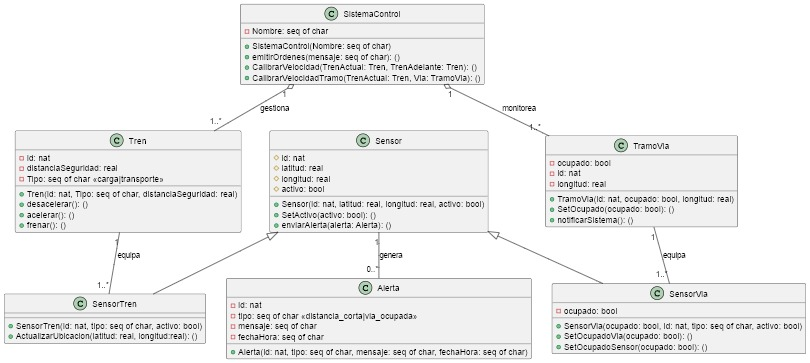
\includegraphics[width=0.48\textwidth]{img/diagrama-clases.jpg}
    \caption{Modelo de datos generado por VDM}
    \label{fig:VDM_model}
\end{figure}


%CLASE ALERTA
    \subsubsection*{Clase \texttt{Alerta}}

    La clase \texttt{Alerta} representa una alerta del sistema con información relevante sobre su tipo, mensaje, fecha y hora de ocurrencia. Esta clase incluye los siguientes atributos privados:

    \begin{itemize}
    \item \texttt{idAlert}: Identificador numérico único de la alerta (tipo \texttt{nat1}).
    \item \texttt{typeAlert}: Tipo de la alerta como una secuencia de caracteres (\texttt{seq of char}).
    \item \texttt{messageAlert}: Mensaje descriptivo de la alerta (\texttt{seq of char}).
    \item \texttt{dateAlert}: Fecha de la alerta, representada como una tupla \texttt{(día, mes, año)} de tipo \texttt{nat1 * nat1 * nat1}.
    \item \texttt{hourAlert}: Hora de la alerta, representada como una tupla \texttt{(hora, minuto, segundo)} de tipo \texttt{nat * nat * nat}.
    \end{itemize}

    La clase proporciona un único constructor público:

    \begin{quote}
    \texttt{Alerta: nat1 * seq of char * seq of char * (nat1 * nat1 * nat1) * (nat * nat * nat) \texttt{==>} Alerta}
    \end{quote}

    El constructor inicializa todos los campos privados a partir de los valores proporcionados como argumentos:
    \begin{itemize}
    \item \texttt{identificadorAlerta} $\rightarrow$ \texttt{idAlert}
    \item \texttt{tipoAlerta} $\rightarrow$ \texttt{typeAlert}
    \item \texttt{mensageAlerta} $\rightarrow$ \texttt{messageAlert}
    \item \texttt{diaAlerta} $\rightarrow$ \texttt{dateAlert}
    \item \texttt{horaAlerta} $\rightarrow$ \texttt{hourAlert}
    \end{itemize}

\lstinputlisting[language=VMDPP,caption={Alerta.vpp}, label={lst:vpp-codigo}]{../vdm++/Alerta.vpp}

%CLASE SENSOR
    \subsubsection*{Clase \texttt{Sensor}}

    La clase \texttt{Sensor} representa un sensor genérico dentro del sistema, encapsulando información básica sobre su identidad y estado operativo. Esta clase incluye los siguientes atributos protegidos:

    \begin{itemize}
    \item \texttt{idSensor}: Identificador numérico único del sensor (tipo \texttt{nat1}).
    \item \texttt{assetSensor}: Indicador booleano del estado del sensor: \texttt{true} si está activo, \texttt{false} en caso contrario.
    \end{itemize}

    La clase proporciona un constructor público:

    \begin{quote}
    \texttt{Sensor: nat1 * bool \texttt{==>} Sensor}
    \end{quote}

    El constructor inicializa los campos protegidos con los valores proporcionados como argumentos:

    \begin{itemize}
    \item \texttt{identificadorSensor} $\rightarrow$ \texttt{idSensor}
    \item \texttt{activoSensor} $\rightarrow$ \texttt{assetSensor}
    \end{itemize}

\lstinputlisting[language=VMDPP,caption={Sensor.vpp}, label={lst:vpp-codigo}]{../vdm++/Sensor.vpp}

%CLASE SensorDeProximidad

    \subsubsection*{Clase \texttt{SensorDeProximidad}}

    La clase \texttt{SensorDeProximidad} es una subclase de \texttt{Sensor} y extiende sus funcionalidades al incluir información sobre la detección y el objeto detectado. Esta clase introduce dos nuevas variables de instancia privadas:

    \begin{itemize}
    \item \texttt{detection}: Estado de la detección, indicando si el sensor ha detectado un objeto (tipo \texttt{bool}).
    \item \texttt{thatIsDetected}: Descripción del objeto detectado, representada como una secuencia de caracteres (\texttt{seq of char}).
    \end{itemize}

    La clase incluye un constructor público:

    \begin{quote}
    \texttt{SensorDeProximidad: nat1 * bool * bool * seq of char \texttt{==>} SensorDeProximidad}
    \end{quote}

    El constructor recibe los siguientes parámetros:
    \begin{itemize}
    \item \texttt{identificadorSensor} $\rightarrow$ \texttt{idSensor}
    \item \texttt{activoSensor} $\rightarrow$ \texttt{assetSensor}
    \item \texttt{deteccion} $\rightarrow$ \texttt{detection}
    \item \texttt{queSeDetecta} $\rightarrow$ \texttt{thatIsDetected}
    \end{itemize}

\lstinputlisting[language=VMDPP,caption={SensorDeProximidad.vpp}, label={lst:vpp-codigo}]{../vdm++/SensorDeProximidad.vpp}

%CLASE SensorEntreTrenes

    \subsubsection*{Clase \texttt{SensorEntreTrenes}}

    La clase \texttt{SensorEntreTrenes} es una subclase de \texttt{Sensor} que extiende su funcionalidad al incluir información adicional sobre la distancia con el tren delantero y la existencia de otro tren en la vía. Esta clase contiene las siguientes variables de instancia privadas:

    \begin{itemize}
    \item \texttt{distanceWithFrontTrain}: Distancia con el tren delantero, medida en unidades reales (tipo \texttt{real}).
    \item \texttt{existsTrain}: Estado que indica si existe un tren en la vía (tipo \texttt{bool}).
    \end{itemize}

    El constructor público de la clase \texttt{SensorEntreTrenes} se define como:

    \begin{quote}
    \texttt{SensorEntreTrenes: nat1 * bool * real * bool \texttt{==>} SensorEntreTrenes}
    \end{quote}

    El constructor inicializa las variables de instancia a partir de los parámetros proporcionados:
    \begin{itemize}
    \item \texttt{identificadorSensor} $\rightarrow$ \texttt{idSensor}
    \item \texttt{activoSensor} $\rightarrow$ \texttt{assetSensor}
    \item \texttt{distanciaConTrenDelantero} $\rightarrow$ \texttt{distanceWithFrontTrain}
    \item \texttt{existeTren} $\rightarrow$ \texttt{existsTrain}
    \end{itemize}

\lstinputlisting[language=VMDPP,caption={SensorEntreTrenes.vpp}, label={lst:vpp-codigo}]{../vdm++/SensorEntreTrenes.vpp}

%CLASE SistemaControl

    \subsubsection*{Clase \texttt{SistemaControl}}

    La clase \texttt{SistemaControl} representa el sistema de control que gestiona el funcionamiento del conjunto de sensores y alertas. Su única variable de instancia es privada:

    \begin{itemize}
    \item \texttt{name}: Nombre del sistema de control, representado como una secuencia de caracteres (\texttt{seq of char}).
    \end{itemize}

    La clase incluye un constructor público:

    \begin{quote}
    \texttt{SistemaControl: seq of char \texttt{==>} SistemaControl}
    \end{quote}

    El constructor inicializa la variable de instancia \texttt{name} con el valor proporcionado:

    \begin{itemize}
    \item \texttt{nombre} $\rightarrow$ \texttt{name}
    \end{itemize}

\lstinputlisting[language=VMDPP,caption={SistemaControl.vpp}, label={lst:vpp-codigo}]{../vdm++/SistemaControl.vpp}

%CLASE Tren

    \subsubsection*{Clase \texttt{Tren}}

    La clase \texttt{Tren} representa un tren en el sistema. Contiene información sobre su identificador, tipo, longitud y distancia de seguridad. Las variables de instancia de la clase son privadas:

    \begin{itemize}
    \item \texttt{idTrain}: Identificador numérico único del tren (tipo \texttt{nat1}).
    \item \texttt{typeTrain}: Tipo de tren, representado como una secuencia de caracteres (\texttt{seq of char}).
    \item \texttt{lengthTrain}: Longitud del tren en unidades reales (tipo \texttt{real}).
    \item \texttt{distanceSafetyTrain}: Distancia de seguridad del tren, también representada en unidades reales (tipo \texttt{real}).
    \end{itemize}

    El constructor público de la clase \texttt{Tren} es:

    \begin{quote}
    \texttt{Tren: nat1 * seq of char * real * real \texttt{==>} Tren}
    \end{quote}

    Este constructor inicializa las variables de instancia con los valores proporcionados:

    \begin{itemize}
    \item \texttt{identificadorTren} $\rightarrow$ \texttt{idTrain}
    \item \texttt{tipoTren} $\rightarrow$ \texttt{typeTrain}
    \item \texttt{longitudTren} $\rightarrow$ \texttt{lengthTrain}
    \item \texttt{distanciaSeguridadTren} $\rightarrow$ \texttt{distanceSafetyTrain}
    \end{itemize}

\lstinputlisting[language=VMDPP,caption={Tren.vpp}, label={lst:vpp-codigo}]{../vdm++/Tren.vpp}

\subsection{Model checking}

\bibliographystyle{IEEEtran}
\sloppy
\bibliography{citas}

\end{document}
